
%%%%%%%%%%%%%%%%%%%%%%%%%%%%%%%%%%%%%%%%%
% "ModernCV" CV and Cover Letter
% LaTeX Template
% Version 1.11 (19/6/14)
%
% This template has been downloaded from:
% http://www.LaTeXTemplates.com
%
% Original author:
% Xavier Danaux (xdanaux@gmail.com)
%
% License:
% CC BY-NC-SA 3.0 (http://creativecommons.org/licenses/by-nc-sa/3.0/)
%
% Important note:
% This template requires the moderncv.cls and .sty files to be in the same 
% directory as this .tex file. These files provide the resume style and themes 
% used for structuring the document.
%
%%%%%%%%%%%%%%%%%%%%%%%%%%%%%%%%%%%%%%%%%

%----------------------------------------------------------------------------------------
%	PACKAGES AND OTHER DOCUMENT CONFIGURATIONS
%----------------------------------------------------------------------------------------
\documentclass[11pt,a4paper,sans]{moderncv} % Font sizes: 10, 11, or 12; paper sizes: a4paper, letterpaper, a5paper, legalpaper, executivepaper or landscape; font families: sans or roman
\usepackage[utf8]{inputenc}
\usepackage[scale=0.75]{geometry}
%\usepackage[top=0.5cm, bottom=0.5cm, left=1.5cm, right=1.5cm]{geometry} 


\moderncvstyle{banking} % CV theme - options include: 'casual' (default), 'classic', 'oldstyle' and 'banking'
\moderncvcolor{blue} % CV color - options include: 'blue' (default), 'orange', 'green', 'red', 'purple', 'grey' and 'black'

%\usepackage[T1]{fontenc}
\usepackage{parcolumns}
\usepackage{comment}

\makeatletter\renewcommand*{\bibliographyitemlabel}{\@biblabel{\arabic{enumiv}}}\makeatother

%\setlength{\hintscolumnwidth}{3cm} % Uncomment to change the width of the dates column
%\setlength{\makecvtitlenamewidth}{10cm} % For the 'classic' style, uncomment to adjust the width of the space allocated to your name

%----------------------------------------------------------------------------------------
%	NAME AND CONTACT INFORMATION SECTION
%----------------------------------------------------------------------------------------

\firstname{Andrea} % Your first name
\familyname{Brugnoli} % Your last name

%% All information in this block is optional, comment out any lines you don't need
%\address{Via Ca' del Frate 7 E}{Negrar (VR), Italy 37024}
%\mobile{(+39) 340 8323361}
%% \phone{(000) 111 1112}
%% \fax{(000) 111 1113}
%\email{brugnoss.ab@gmail.com}
%% \homepage{staff.org.edu/~jsmith}{staff.org.edu/$\sim$jsmith} % The first argument is the url for the clickable link, the second argument is the url displayed in the template - this allows special characters to be displayed such as the tilde in this example
%\extrainfo{Skype contact: brugnoss}
%\photo[70pt][0.4pt]{pictures/Foto_cv} % The first bracket is the picture height, the second is the thickness of the frame around the picture (0pt for no frame)

\AtBeginDocument{\hypersetup{baseurl={}}}

%----------------------------------------------------------------------------------------

\begin{document}

%\makecvtitle % Print the CV title

\begin{minipage}{.8\linewidth}
{\huge{\textsc{Andrea BRUGNOLI}}}

\vspace{2mm}
{103 rue Bonnat, 31400 Toulouse (FR)}

{(+33) 7 50 39 47 27}

{ Andrea.BRUGNOLI@supaero.isae.fr or andrea.brugnoli92@gmail.com}

\vspace{3mm}
% \homepage{staff.org.edu/~jsmith}{staff.org.edu/$\sim$jsmith} % The first argument is the url for the clickable link, the second argument is the url displayed in the template - this allows special characters to be displayed such as the tilde in this example
%\end{minipage}
%\begin{minipage}{.4\linewidth}

\fcolorbox{cyan}{white}{%
    \parbox{\textwidth}{\textbf{Phd candidate at ISAE-Supaero (Toulouse)} \newline
 \vspace{1mm}
International spirit, initiative and ability to adapt. Fluent in three languages.
  }}
\end{minipage}
\begin{minipage}{.2\linewidth}
\begin{center}
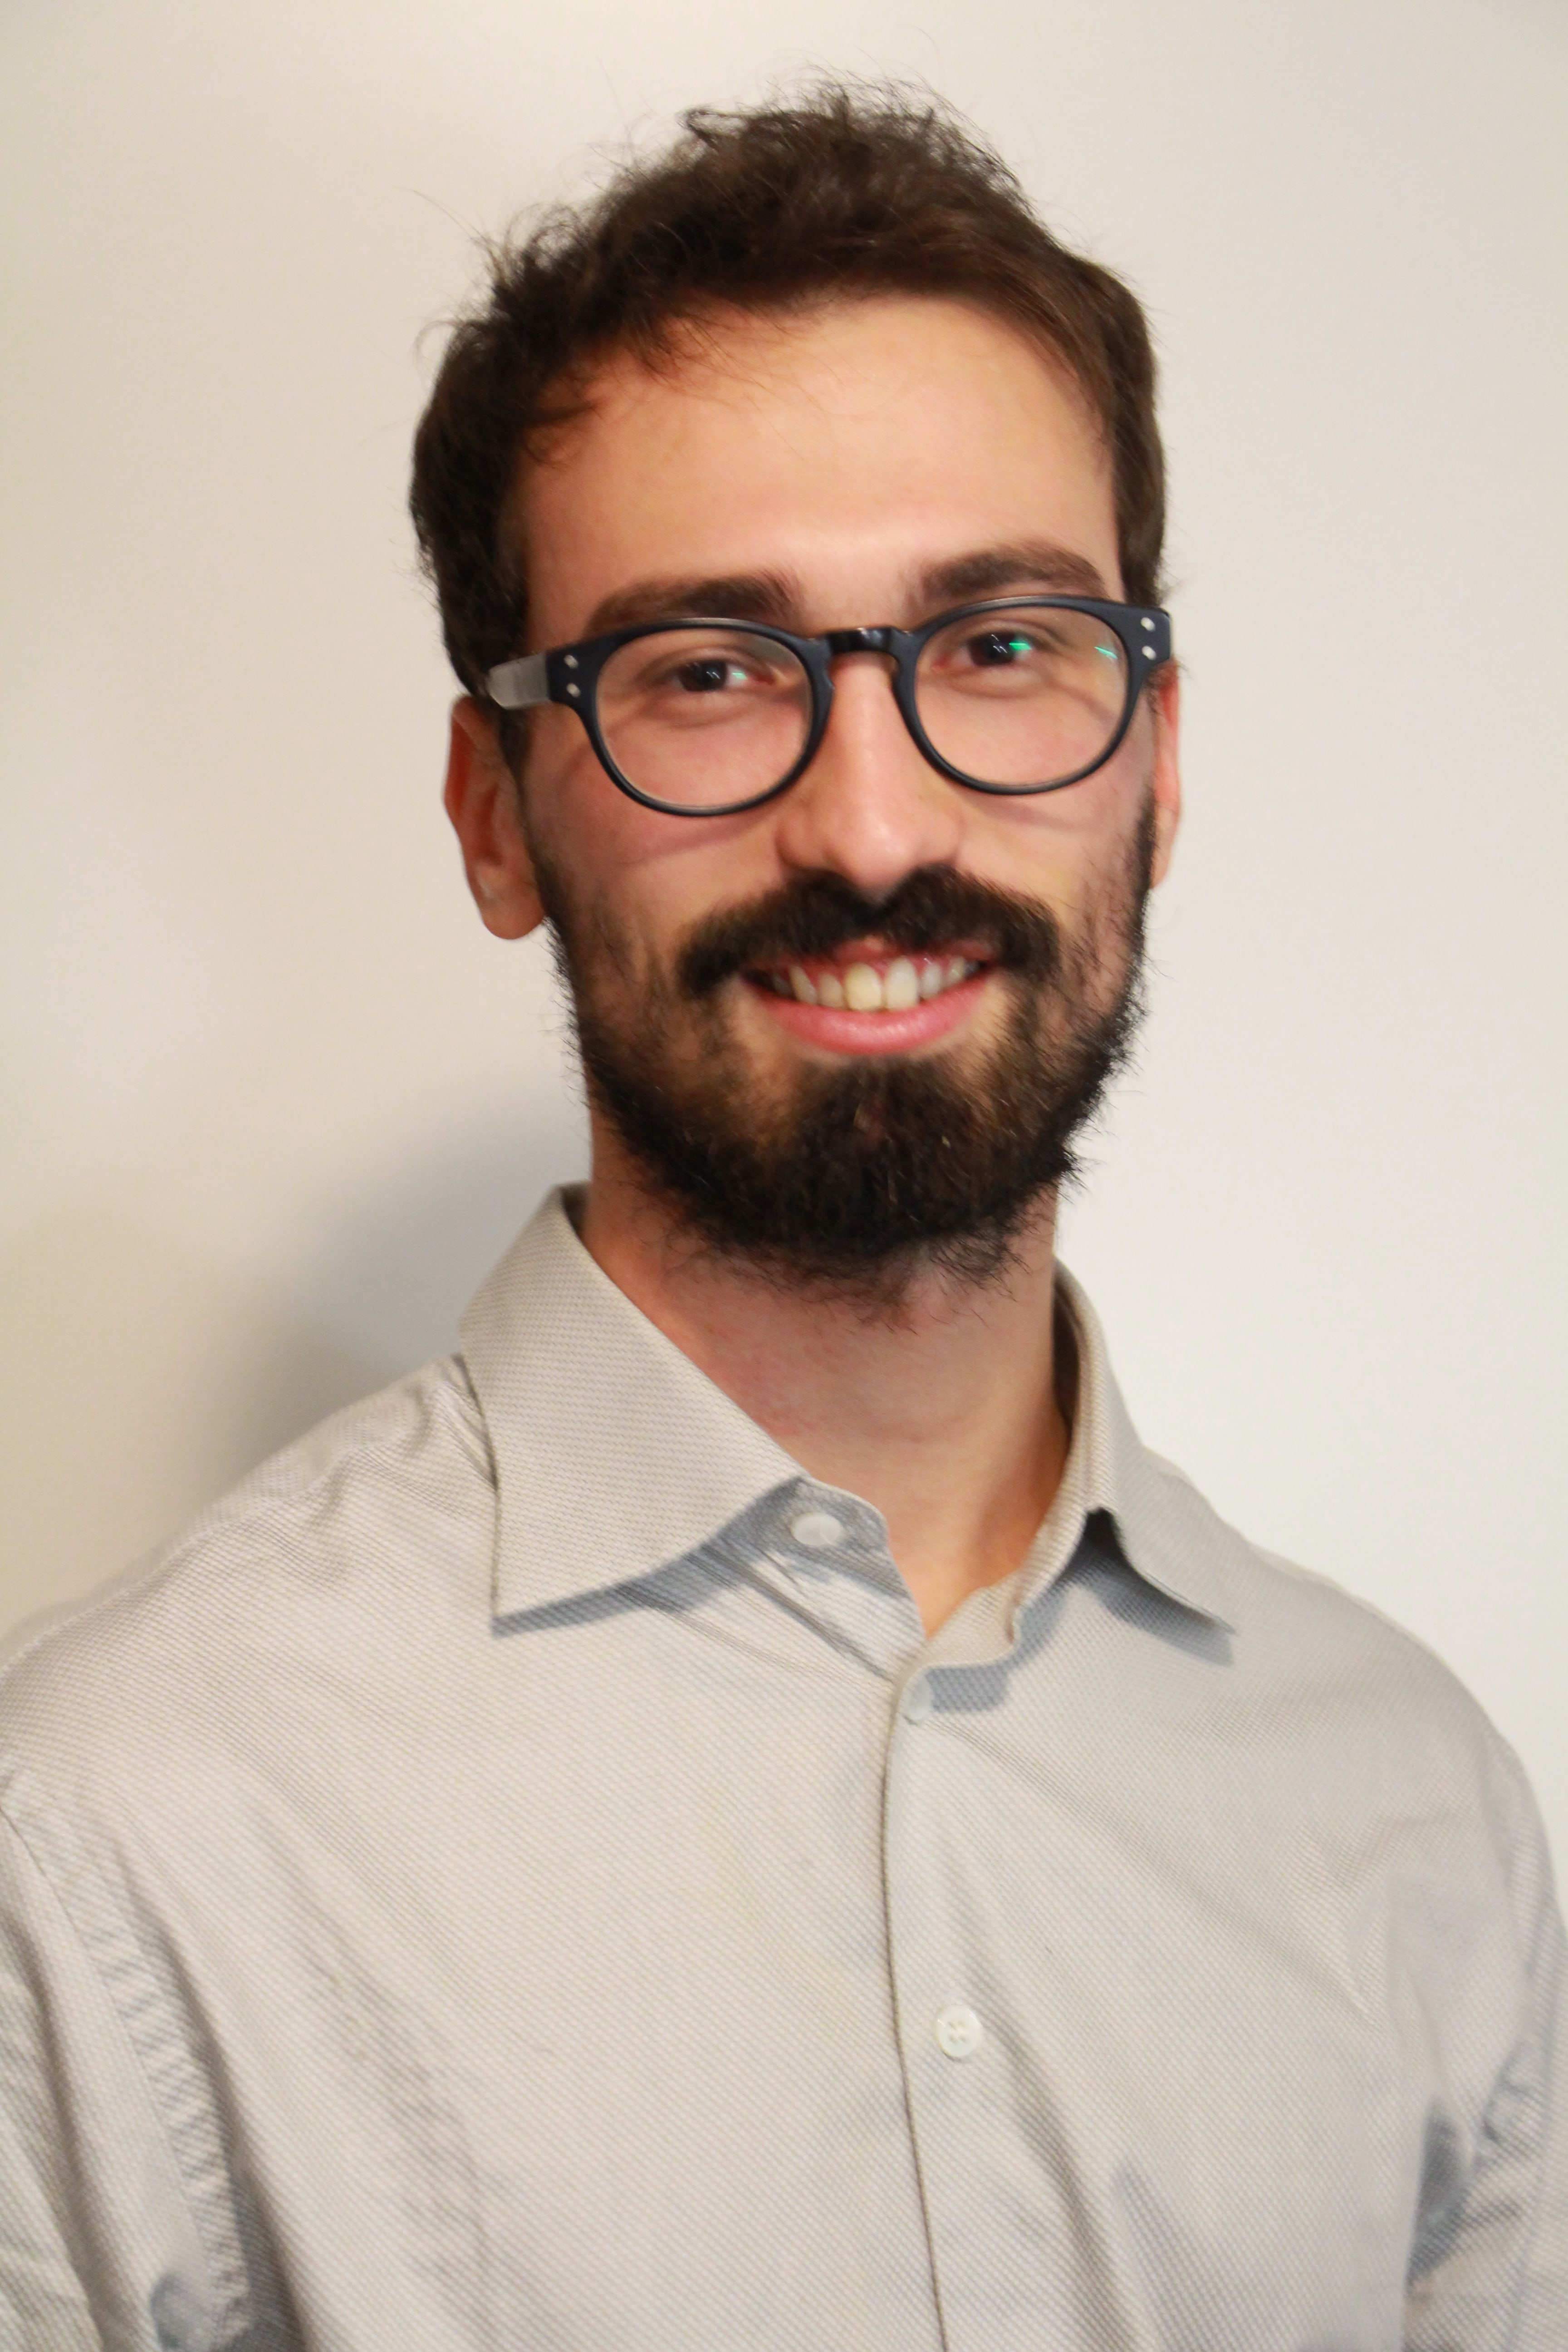
\includegraphics[width=0.8\linewidth]{Foto_Cv-min.jpg}
\end{center}
\end{minipage}

%\vspace{2mm}
% \textbf{Seeking a job from April 2017 in automatics and optimization.}

%----------------------------------------------------------------------------------------
%	EDUCATION SECTION
%----------------------------------------------------------------------------------------

\vspace{3mm}



\section{Education}

% usage: \cventry[spacing]{years}{degree/job title}{institution/employer}{localization}{optionnal: grade/...}{optional: comment/job description}

\cventry{October 2017-October 2020}{PhD candidate}{ISAE-Supaero}{Toulouse}{}{A port-Hamiltonian formulation of flexible structures: modelling and symplectic finite element discretization.}

\cventry{2016--2017}{Research Master in automatics and image processing}{Université Paris Saclay/\,Supélec}{Paris/Toulouse}{}{Courses: inverse problem, advanced dynamics of flexible structures, parameter estimation}

\cventry{2015--2017}{Double degree in aerospace and astronautical engineering}{ISAE-Supaero}{Toulouse}{}{Specialisation in applied mathematics and advanced automatics: multidisciplinary optimisation, high performance computing, control of flexible structures}


\cventry{2014--2017}{Master in space engineering}{Politecnico di Milano}{Milano}{\textit{110/110 cum laude} }{
Courses: orbital mechanics, structural dynamics and control, thermochemical propulsion }


\cventry{2011--2014}{Mechanical Engineering Degree}{Politecnico di Milano}{Milano}{\textit{110/110 cum laude} }{Courses: finite element method, mechanical vibrations, numerical methods for engineering}

%\cventry{2006--2011}{High school diploma}{Liceo Classico Scipione Maffei}{Verona}{\textit{100/100}}{}

\vspace{1mm}

%----------------------------------------------------------------------------------------
%	WORK EXPERIENCE SECTION
%----------------------------------------------------------------------------------------

\section{Experiences}

\cventry{January 2019, 4 months}{Visiting researcher}{ITA-Instituto Tecnol\'{o}gico de Aeron\'{a}utica}{S\~{a}o Jos\'{e} dos Campos}{}{Collaboration with Flavio Cardoso-Riberio on numerical methods for port-Hamiltonian systems (see References).}

\cventry{2017, 6 months}{Internship}{CNES-Centre  des études spatiales}{Toulouse}{}{Analysis of dismissed satellites subject to solar pressure to identify stable pointing configurations and periodical behaviours.}

\cventry{2016, 5 months}{Industrial and entrepreneurial project}{ISAE-Supaero in partnership with LAAS}{Toulouse}{}{Intelligent teleoperations for micro-drones systems (six people team).}

\cventry{2016, 4 months}{Research project}{ISAE-Supaero}{Toulouse}{}{Modular modelling of rigid multibody systems following the logic of Simscape Multibody}

%\cventry{2015, 2 months}{Interplanetary transfer}{Politecnico di Milano}{Milano}{}{\' 
%Study of optimal trajectories with gravity assist to minimise propellant usage. Perturbation analysis on operational orbit.}

\cventry{July 2014, September 2014}{Bachelor project}{Politecnico di Milano in  partnership with Danieli S.p.A}{Milano}{} {Dynamics of a forging manipulator: kinematics modelisation and dynamic analysis. Presented at Danieli.}

%\cventry{2014, 3 months}{Fem analysis of a mechanical component}{Politecnico di Milano}{Milano}{}{Implementation on Abaqus, equivalent model coded on Matlab , results validation and comparison.}

%\cventry{}{Horizontal Axis Wind Turbine Design}{Politecnico di Milano}{Milano}{}{General sizing, performances optimization nominal point, performance analysis off design. Team of four. Published on Academia  \textcolor{blue}{\texttt{\href{https://www.academia.edu/9561531/Horizontal_Axis_Wind_Turbine_Design}{Horizontal Axis Wind Turbine Design}}} }

%\nocite{companion,bertram,cicero,augustine}

\nocite{*}
\bibliographystyle{unsrt}
\bibliography{cv_bibliography}   

%----------------------------------------------------------------------------------------
%	COMPUTER SKILLS SECTION
%----------------------------------------------------------------------------------------

%----------------------------------------------------------------------------------------
%	COMMUNICATION SKILLS SECTION
%----------------------------------------------------------------------------------------

% \section{Communication Skills}

% \cvitem{2010}{Oral Presentation at the California Business Conference}
% \cvitem{2009}{Poster at the Annual Business Conference in Oregon}

%----------------------------------------------------------------------------------------
%	LANGUAGES SECTION
%----------------------------------------------------------------------------------------
\begin{minipage}[t]{0.4\linewidth}
\section{Languages}
\cvitem{English}{fluent (Toeic 965/990 2014)}
\cvitem{French}{fluent}
\cvitem{Spanish}{intermediate}
\cvitem{Brazilian portuguese}{intermediate}
\cvitem{Italian}{native speaker}
\end{minipage}
\begin{minipage}[t]{0.5\linewidth}
\section{Computer skills}
\cvitem{Softwares and platforms}{Simulink, Abaqus, Inventor, Solid Works, Labview}
\cvitem{Languages}{Python (especially FEM librairies: FEniCS and Firedrake), Matlab, Java, C, \LaTeX}
\end{minipage}


\begin{comment}
\section{Languages}
\begin{minipage}{0.45\linewidth}
\cvitem{}{English: fluent (Toeic 965/990 2014)}
\cvitem{}{French: fluent}
\end{minipage}
\textcolor{color1}{\vrule width 0.3pt}
\begin{minipage}{0.45\linewidth}
\quad \cvitem{}{Spanish: good command}
\quad \cvitem{}{Italian: native speaker}
\end{minipage}
\end{comment}



%----------------------------------------------------------------------------------------
%	INTERESTS SECTION
%----------------------------------------------------------------------------------------

\section{Interests}

\cvitem{}{Tutor of mathematics and physics for first and second year bachelor students}
\cvitem{}{Tennis, travelling, literature and cinema}



\end{document}










